%
%to crop the pdf, use
% pdfcrop --margins '0 50 0 50' figlayered.pdf figlayered2.pdf
% 


\NeedsTeXFormat{LaTeX2e}
%
%\documentclass[aps,pra,showpacs,amsmath,amssymb,superscriptaddress,nofootinbib]{revtex4}
\documentclass[]{article}
\usepackage{graphicx}% Include figure files
\usepackage{bm}% bold math
\usepackage{amssymb}
\usepackage{amsmath}
\usepackage{latexsym}
\usepackage{color}
\usepackage{soul}
\usepackage{nopageno}
\usepackage{tikz}
%%

\begin{document}  

\thispagestyle{empty}

% figure created using https://www.mathcha.io/editor#

%%%%%%%%%%%%%%%%%%%%%%%%%%%%%%%%  put here figure %%%%%%%%%%%%%%%%%%%%%%%%%%%%%%%%%%%%%%%%%%%%%%%%
\tikzset{every picture/.style={line width=0.75pt}} %set default line width to 0.75pt        

\begin{figure}\label{fig:frame}



% \tikzset{every picture/.style={line width=0.75pt}} %set default line width to 0.75pt        

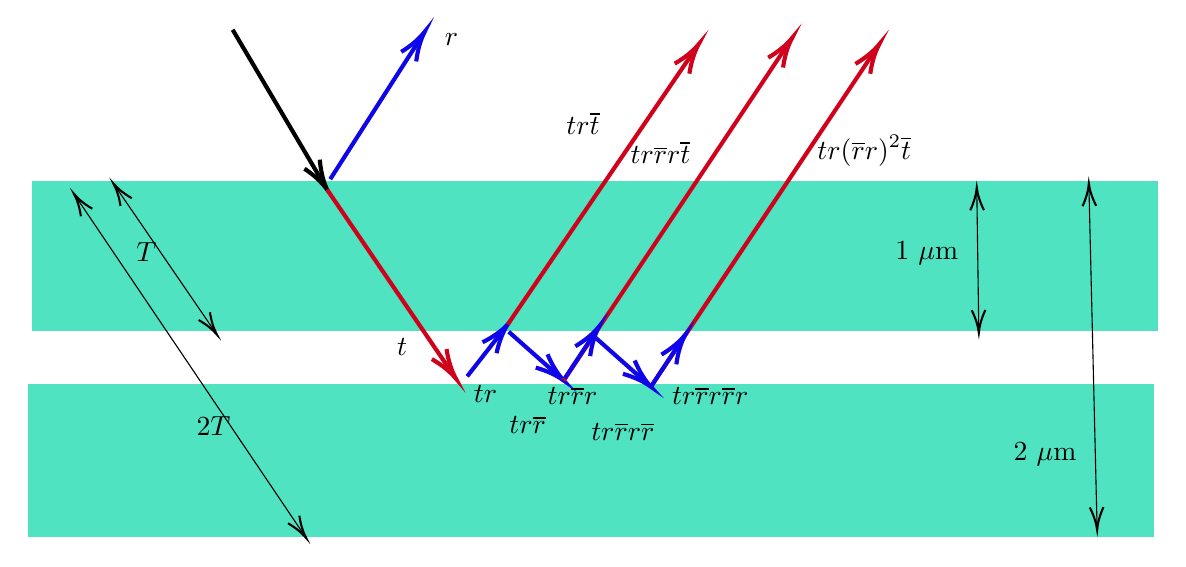
\begin{tikzpicture}[x=0.75pt,y=0.75pt,yscale=-1,xscale=1]
%uncomment if require: \path (0,298); %set diagram left start at 0, and has height of 298

%Shape: Rectangle [id:dp11132417261061733] 
\draw  [color={rgb, 255:red, 80; green, 227; blue, 194 }  ,draw opacity=1 ][fill={rgb, 255:red, 80; green, 227; blue, 194 }  ,fill opacity=1 ] (52.5,88) -- (594.5,88) -- (594.5,160) -- (52.5,160) -- cycle ;
%Straight Lines [id:da575301150571319] 
\draw [line width=1.5]    (149,15) -- (192.97,89.42) ;
\draw [shift={(194.5,92)}, rotate = 239.42] [color={rgb, 255:red, 0; green, 0; blue, 0 }  ][line width=1.5]    (14.21,-4.28) .. controls (9.04,-1.82) and (4.3,-0.39) .. (0,0) .. controls (4.3,0.39) and (9.04,1.82) .. (14.21,4.28)   ;
%Straight Lines [id:da7996585837315047] 
\draw [color={rgb, 255:red, 15; green, 5; blue, 233 }  ,draw opacity=1 ][line width=1.5]    (196,87) -- (239.88,18.53) ;
\draw [shift={(241.5,16)}, rotate = 122.65] [color={rgb, 255:red, 15; green, 5; blue, 233 }  ,draw opacity=1 ][line width=1.5]    (14.21,-4.28) .. controls (9.04,-1.82) and (4.3,-0.39) .. (0,0) .. controls (4.3,0.39) and (9.04,1.82) .. (14.21,4.28)   ;
%Straight Lines [id:da08369442419602358] 
\draw [color={rgb, 255:red, 15; green, 5; blue, 233 }  ,draw opacity=1 ][line width=1.5]    (262,182) -- (279.65,159.37) ;
\draw [shift={(281.5,157)}, rotate = 127.95] [color={rgb, 255:red, 15; green, 5; blue, 233 }  ,draw opacity=1 ][line width=1.5]    (14.21,-4.28) .. controls (9.04,-1.82) and (4.3,-0.39) .. (0,0) .. controls (4.3,0.39) and (9.04,1.82) .. (14.21,4.28)   ;
%Shape: Rectangle [id:dp7208008023108876] 
\draw  [color={rgb, 255:red, 80; green, 227; blue, 194 }  ,draw opacity=1 ][fill={rgb, 255:red, 80; green, 227; blue, 194 }  ,fill opacity=1 ] (50.5,186) -- (592.5,186) -- (592.5,259) -- (50.5,259) -- cycle ;
%Straight Lines [id:da39109169227709817] 
\draw [color={rgb, 255:red, 208; green, 2; blue, 27 }  ,draw opacity=1 ][line width=1.5]    (194.5,92) -- (254.81,180.52) ;
\draw [shift={(256.5,183)}, rotate = 235.73] [color={rgb, 255:red, 208; green, 2; blue, 27 }  ,draw opacity=1 ][line width=1.5]    (14.21,-4.28) .. controls (9.04,-1.82) and (4.3,-0.39) .. (0,0) .. controls (4.3,0.39) and (9.04,1.82) .. (14.21,4.28)   ;
%Straight Lines [id:da07625434489085259] 
\draw [color={rgb, 255:red, 208; green, 2; blue, 27 }  ,draw opacity=1 ][line width=1.5]    (281.5,157) -- (371.81,24.48) ;
\draw [shift={(373.5,22)}, rotate = 124.27] [color={rgb, 255:red, 208; green, 2; blue, 27 }  ,draw opacity=1 ][line width=1.5]    (14.21,-4.28) .. controls (9.04,-1.82) and (4.3,-0.39) .. (0,0) .. controls (4.3,0.39) and (9.04,1.82) .. (14.21,4.28)   ;
%Straight Lines [id:da5266654373833295] 
\draw [color={rgb, 255:red, 15; green, 5; blue, 233 }  ,draw opacity=1 ][line width=1.5]    (282,160.5) -- (306.26,182.01) ;
\draw [shift={(308.5,184)}, rotate = 221.57] [color={rgb, 255:red, 15; green, 5; blue, 233 }  ,draw opacity=1 ][line width=1.5]    (14.21,-4.28) .. controls (9.04,-1.82) and (4.3,-0.39) .. (0,0) .. controls (4.3,0.39) and (9.04,1.82) .. (14.21,4.28)   ;
%Straight Lines [id:da08063995785013289] 
\draw [color={rgb, 255:red, 208; green, 2; blue, 27 }  ,draw opacity=1 ][line width=1.5]    (308.5,184) -- (416.84,21.5) ;
\draw [shift={(418.5,19)}, rotate = 123.69] [color={rgb, 255:red, 208; green, 2; blue, 27 }  ,draw opacity=1 ][line width=1.5]    (14.21,-4.28) .. controls (9.04,-1.82) and (4.3,-0.39) .. (0,0) .. controls (4.3,0.39) and (9.04,1.82) .. (14.21,4.28)   ;
%Straight Lines [id:da5326424820591018] 
\draw [color={rgb, 255:red, 15; green, 5; blue, 233 }  ,draw opacity=1 ][line width=1.5]    (324,163.5) -- (348.26,185.01) ;
\draw [shift={(350.5,187)}, rotate = 221.57] [color={rgb, 255:red, 15; green, 5; blue, 233 }  ,draw opacity=1 ][line width=1.5]    (14.21,-4.28) .. controls (9.04,-1.82) and (4.3,-0.39) .. (0,0) .. controls (4.3,0.39) and (9.04,1.82) .. (14.21,4.28)   ;
%Straight Lines [id:da3207009815189019] 
\draw [color={rgb, 255:red, 208; green, 2; blue, 27 }  ,draw opacity=1 ][line width=1.5]    (350.5,187) -- (458.84,24.5) ;
\draw [shift={(460.5,22)}, rotate = 123.69] [color={rgb, 255:red, 208; green, 2; blue, 27 }  ,draw opacity=1 ][line width=1.5]    (14.21,-4.28) .. controls (9.04,-1.82) and (4.3,-0.39) .. (0,0) .. controls (4.3,0.39) and (9.04,1.82) .. (14.21,4.28)   ;
%Straight Lines [id:da013199287023920148] 
\draw [color={rgb, 255:red, 15; green, 5; blue, 233 }  ,draw opacity=1 ][line width=1.5]    (309,183) -- (323.85,160.5) ;
\draw [shift={(325.5,158)}, rotate = 123.42] [color={rgb, 255:red, 15; green, 5; blue, 233 }  ,draw opacity=1 ][line width=1.5]    (14.21,-4.28) .. controls (9.04,-1.82) and (4.3,-0.39) .. (0,0) .. controls (4.3,0.39) and (9.04,1.82) .. (14.21,4.28)   ;
%Straight Lines [id:da4112765567049961] 
\draw [color={rgb, 255:red, 15; green, 5; blue, 233 }  ,draw opacity=1 ][line width=1.5]    (350.5,187) -- (365.35,164.5) ;
\draw [shift={(367,162)}, rotate = 123.42] [color={rgb, 255:red, 15; green, 5; blue, 233 }  ,draw opacity=1 ][line width=1.5]    (14.21,-4.28) .. controls (9.04,-1.82) and (4.3,-0.39) .. (0,0) .. controls (4.3,0.39) and (9.04,1.82) .. (14.21,4.28)   ;
%Straight Lines [id:da32280483055720977] 
\draw    (92.63,90.65) -- (140.37,160.35) ;
\draw [shift={(141.5,162)}, rotate = 235.59] [color={rgb, 255:red, 0; green, 0; blue, 0 }  ][line width=0.75]    (10.93,-3.29) .. controls (6.95,-1.4) and (3.31,-0.3) .. (0,0) .. controls (3.31,0.3) and (6.95,1.4) .. (10.93,3.29)   ;
\draw [shift={(91.5,89)}, rotate = 55.59] [color={rgb, 255:red, 0; green, 0; blue, 0 }  ][line width=0.75]    (10.93,-3.29) .. controls (6.95,-1.4) and (3.31,-0.3) .. (0,0) .. controls (3.31,0.3) and (6.95,1.4) .. (10.93,3.29)   ;
%Straight Lines [id:da8957499355816798] 
\draw    (73.62,95.66) -- (183.38,258.34) ;
\draw [shift={(184.5,260)}, rotate = 235.99] [color={rgb, 255:red, 0; green, 0; blue, 0 }  ][line width=0.75]    (10.93,-3.29) .. controls (6.95,-1.4) and (3.31,-0.3) .. (0,0) .. controls (3.31,0.3) and (6.95,1.4) .. (10.93,3.29)   ;
\draw [shift={(72.5,94)}, rotate = 55.99] [color={rgb, 255:red, 0; green, 0; blue, 0 }  ][line width=0.75]    (10.93,-3.29) .. controls (6.95,-1.4) and (3.31,-0.3) .. (0,0) .. controls (3.31,0.3) and (6.95,1.4) .. (10.93,3.29)   ;
%Straight Lines [id:da5367146347196039] 
\draw    (507.53,93) -- (508.47,159) ;
\draw [shift={(508.5,161)}, rotate = 269.18] [color={rgb, 255:red, 0; green, 0; blue, 0 }  ][line width=0.75]    (10.93,-3.29) .. controls (6.95,-1.4) and (3.31,-0.3) .. (0,0) .. controls (3.31,0.3) and (6.95,1.4) .. (10.93,3.29)   ;
\draw [shift={(507.5,91)}, rotate = 89.18] [color={rgb, 255:red, 0; green, 0; blue, 0 }  ][line width=0.75]    (10.93,-3.29) .. controls (6.95,-1.4) and (3.31,-0.3) .. (0,0) .. controls (3.31,0.3) and (6.95,1.4) .. (10.93,3.29)   ;
%Straight Lines [id:da5859148060151764] 
\draw    (561.55,91) -- (565.45,254) ;
\draw [shift={(565.5,256)}, rotate = 268.63] [color={rgb, 255:red, 0; green, 0; blue, 0 }  ][line width=0.75]    (10.93,-3.29) .. controls (6.95,-1.4) and (3.31,-0.3) .. (0,0) .. controls (3.31,0.3) and (6.95,1.4) .. (10.93,3.29)   ;
\draw [shift={(561.5,89)}, rotate = 88.63] [color={rgb, 255:red, 0; green, 0; blue, 0 }  ][line width=0.75]    (10.93,-3.29) .. controls (6.95,-1.4) and (3.31,-0.3) .. (0,0) .. controls (3.31,0.3) and (6.95,1.4) .. (10.93,3.29)   ;

% Text Node
\draw (250,15.67) node [anchor=north west][inner sep=0.75pt]   [align=left] {$\displaystyle r$};
% Text Node
\draw (101.33,116.33) node [anchor=north west][inner sep=0.75pt]   [align=left] {$\displaystyle T$};
% Text Node
\draw (227,162.67) node [anchor=north west][inner sep=0.75pt]   [align=left] {$\displaystyle t$};
% Text Node
\draw (264,185) node [anchor=north west][inner sep=0.75pt]   [align=left] {$\displaystyle tr$};
% Text Node
\draw (308.5,53.5) node [anchor=north west][inner sep=0.75pt]   [align=left] {$\displaystyle tr\overline{t}$};
% Text Node
\draw (339.5,67.5) node [anchor=north west][inner sep=0.75pt]   [align=left] {$\displaystyle tr\overline{r} r\overline{t}$};
% Text Node
\draw (429.5,64.5) node [anchor=north west][inner sep=0.75pt]   [align=left] {$\displaystyle tr(\overline{r} r)^{2}\overline{t}$};
% Text Node
\draw (281,200) node [anchor=north west][inner sep=0.75pt]   [align=left] {$\displaystyle tr\overline{r}$};
% Text Node
\draw (299.5,186) node [anchor=north west][inner sep=0.75pt]   [align=left] {$\displaystyle tr\overline{r} r$};
% Text Node
\draw (130.33,200.33) node [anchor=north west][inner sep=0.75pt]   [align=left] {$\displaystyle 2T$};
% Text Node
\draw (467,115.67) node [anchor=north west][inner sep=0.75pt]   [align=left] {1 $\displaystyle \mu $m};
% Text Node
\draw (524,212.67) node [anchor=north west][inner sep=0.75pt]   [align=left] {2 $\displaystyle \mu $m};
% Text Node
\draw (320.5,203) node [anchor=north west][inner sep=0.75pt]   [align=left] {$\displaystyle tr\overline{r} r\overline{r}$};
% Text Node
\draw (359.5,186) node [anchor=north west][inner sep=0.75pt]   [align=left] {$\displaystyle tr\overline{r} r\overline{r} r$};


\end{tikzpicture}


\end{figure}

%%%%%%%%%%%%%%%%%%%%%%%%%%%%%%%%  end put here figure %%%%%%%%%%%%%%%%%%%%%%%%%%%%%%%%%%%%%%%%%%%%%%%%

\end{document}